\documentclass[12pt, twoside]{article}
\usepackage[francais]{babel}
\usepackage[T1]{fontenc}
\usepackage[latin1]{inputenc}
\usepackage[left=7mm, right=7mm, top=7mm, bottom=7mm]{geometry}
\usepackage{float}
\usepackage{graphicx}
\usepackage{array}
\usepackage{multirow}
\usepackage{amsmath,amssymb,mathrsfs}
\usepackage{soul}
\usepackage{textcomp}
\usepackage{eurosym}
 \usepackage{variations}
\usepackage{tabvar}

\pagestyle{empty}

\begin{document}

\begin{flushleft}
NOM PRENOM: \ldots \ldots \ldots \ldots \ldots \ldots \ldots \ldots \ldots
 
\bigskip

\end{flushleft}

\begin{center}
{\fbox{$6^{e}\ldots$ \qquad \qquad \textbf{\Large{Mini-test 1 (sujet 1)}}
\qquad \qquad \ldots/11/2014}}
\end{center}



\bigskip 


\ul{Exercice 1}: 

\begin{tabular}{cc}
\begin{minipage}{11cm}
\begin{enumerate}
  \item Tracer en bleu la droite passant par les points C et A.
  \item Tracer [AB] (en noir).
  \item Tracer [CB) (en vert).
\end{enumerate}
\end{minipage}
&
\begin{minipage}{7cm}
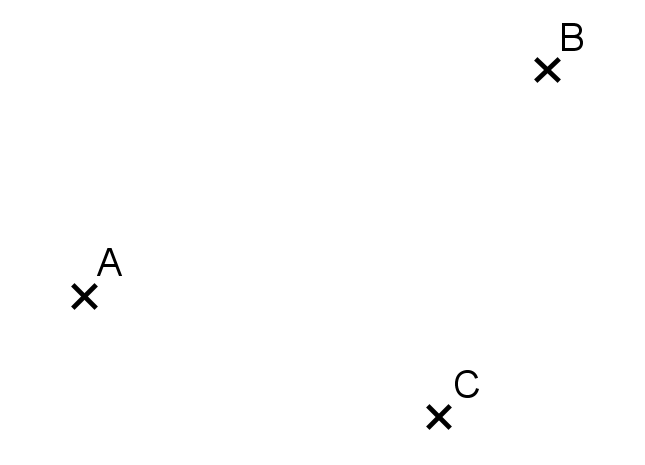
\includegraphics[width=5cm]{images/ex1.png}
\end{minipage}
\end{tabular}

\bigskip

\bigskip


\ul{Exercice 2}: Dans chaque cas, �crire avec les notations math�matiques.

\begin{enumerate}
  \item La demi-droite d'origine F passant par E \qquad \ldots \ldots \ldots
  \ldots \ldots
  \item Le segment d'extr�mit�s V et T \qquad \ldots \ldots \ldots \ldots \ldots
\end{enumerate}

\bigskip

\bigskip

\ul{Exercice 3}: Compl�ter par $\in$ ou $\notin$.

\begin{tabular}{cc}
\begin{minipage}{8cm}
\begin{enumerate}
  \item Q \ldots \ldots [PR]
  \item P \ldots \ldots (QP)
  \item Q \ldots \ldots [RS)
\end{enumerate}
\end{minipage}
&
\begin{minipage}{8cm}
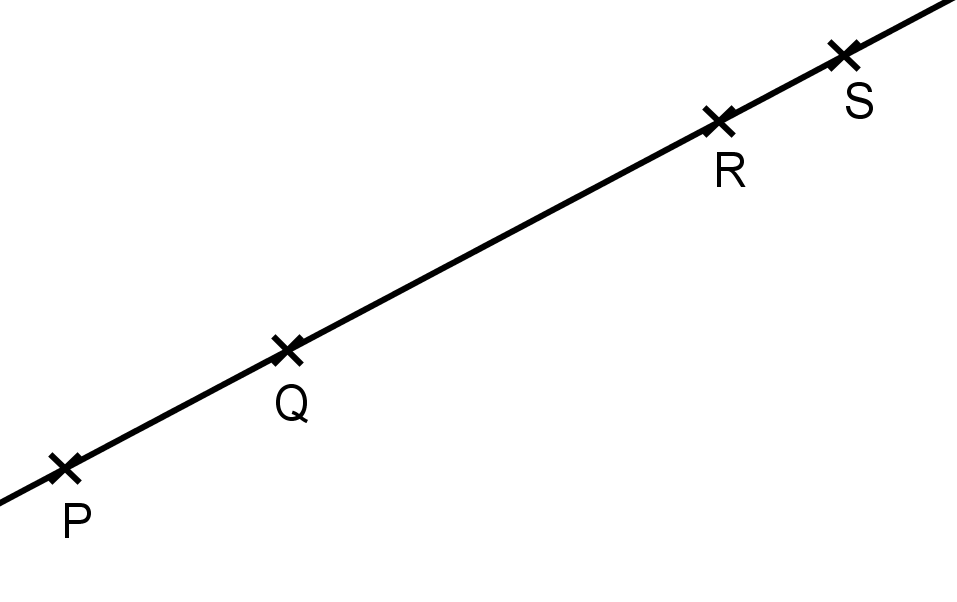
\includegraphics[width=5cm]{images/ex3.png}
\end{minipage}
\end{tabular}

\bigskip

\bigskip

\ul{Exercice 4}: 
Compl�ter les phrases.

\enskip

\begin{tabular}{cc}
\begin{minipage}{12cm}
Les droites $(d_1)$ et $(d_2)$ se coupent en B. On dit aussi que les droites
$(d_1)$ et $(d_2)$ sont \ldots \ldots \ldots \ldots \ldots \ldots \ldots en B.
Le point B est le point \ldots \ldots \ldots \ldots \ldots \ldots \ldots \ldots
\ldots des droites $(d_1)$ et $(d_2)$.
\end{minipage} 
&
\begin{minipage}{6cm}
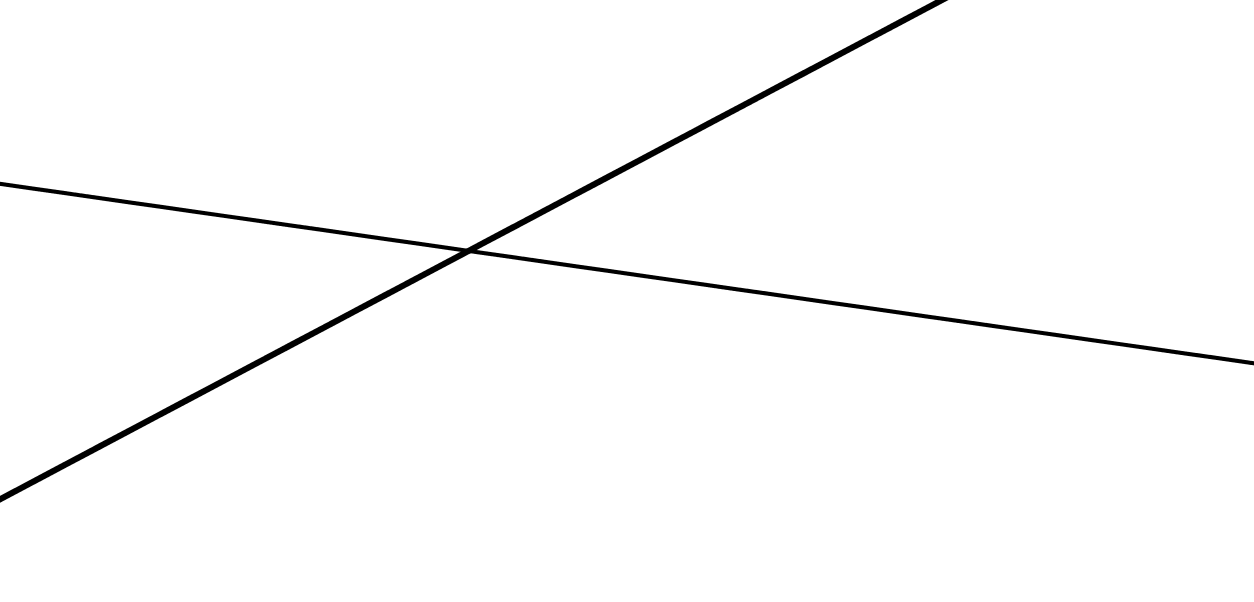
\includegraphics[width=5cm]{images/ex4.png}
\end{minipage}
\end{tabular}


\pagebreak





\begin{flushleft}
NOM PRENOM: \ldots \ldots \ldots \ldots \ldots \ldots \ldots \ldots \ldots
 
\bigskip

\end{flushleft}

\begin{center}
{\fbox{$6^{e}\ldots$ \qquad \qquad \textbf{\Large{Mini-test 1 (sujet 2)}}
\qquad \qquad \ldots/11/2014}}
\end{center}



\bigskip 


\ul{Exercice 1}: 

\begin{tabular}{cc}
\begin{minipage}{11cm}
\begin{enumerate}
  \item Tracer en bleu la droite passant par les points D et E.
  \item Tracer [EF] (en noir).
  \item Tracer [FD) (en vert).
\end{enumerate}
\end{minipage}
&
\begin{minipage}{7cm}
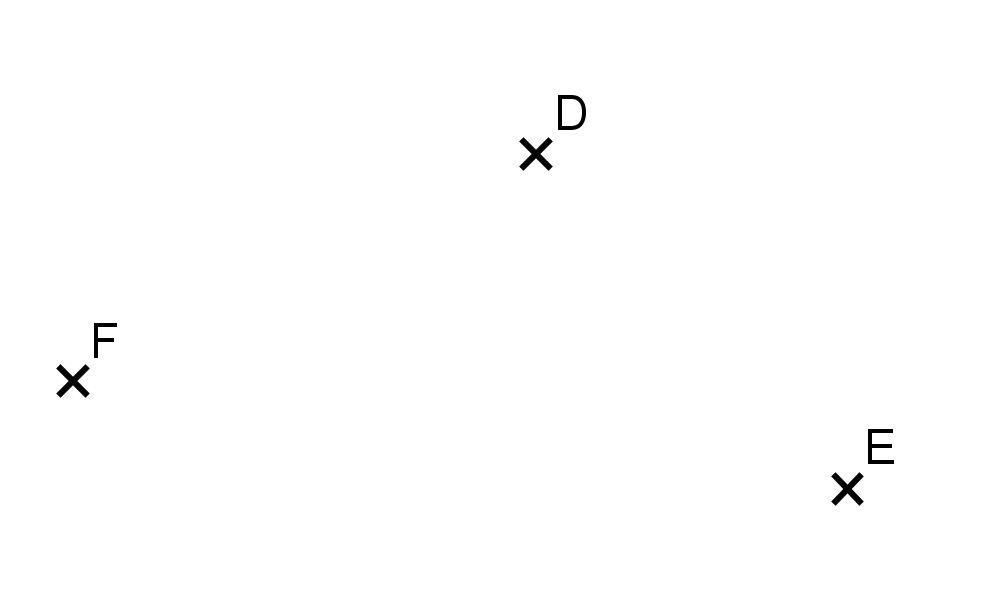
\includegraphics[width=5cm]{images/ex11.png}
\end{minipage}
\end{tabular}

\bigskip

\bigskip


\ul{Exercice 2}: Dans chaque cas, �crire avec les notations math�matiques.

\begin{enumerate}
  \item La demi-droite d'origine U passant par S \qquad \ldots \ldots \ldots
  \ldots \ldots
  \item Le segment d'extr�mit�s G et H \qquad \ldots \ldots \ldots \ldots \ldots
\end{enumerate}

\bigskip

\bigskip

\ul{Exercice 3}: Compl�ter par $\in$ ou $\notin$.

\begin{tabular}{cc}
\begin{minipage}{8cm}
\begin{enumerate}
  \item S \ldots \ldots [PR]
  \item P \ldots \ldots (RP)
  \item P \ldots \ldots [QR)
\end{enumerate}
\end{minipage}
&
\begin{minipage}{8cm}
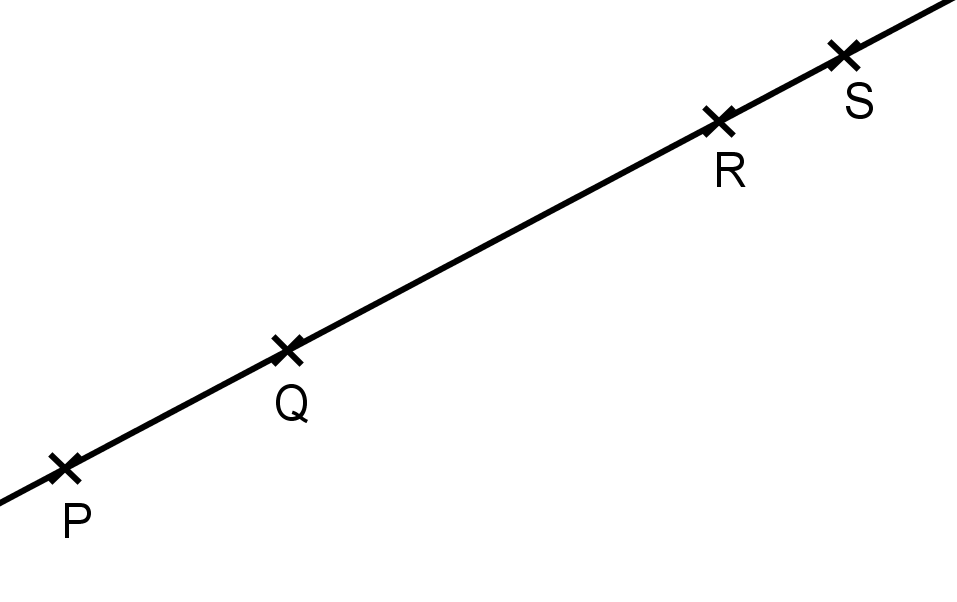
\includegraphics[width=5cm]{images/ex3.png}
\end{minipage}
\end{tabular}

\bigskip

\bigskip

\ul{Exercice 4}: 
Compl�ter les phrases.

\enskip

\begin{tabular}{cc}
\begin{minipage}{12cm}
Les droites $(d_1)$ et $(d_2)$ se coupent en B. On dit aussi que les droites
$(d_1)$ et $(d_2)$ sont \ldots \ldots \ldots \ldots \ldots \ldots \ldots en B.
Le point B est le point \ldots \ldots \ldots \ldots \ldots \ldots \ldots \ldots
\ldots des droites $(d_1)$ et $(d_2)$.
\end{minipage} 
&
\begin{minipage}{6cm}
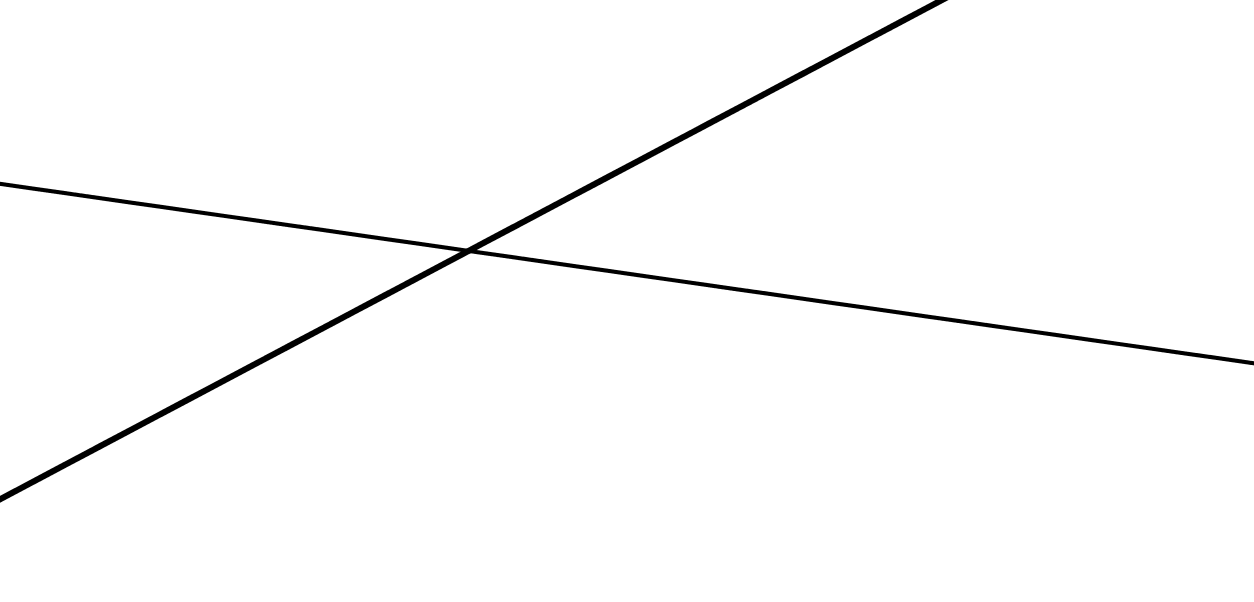
\includegraphics[width=5cm]{images/ex4.png}
\end{minipage}
\end{tabular}

\pagebreak


\quad 
\end{document}
